\section{Introducción}

Las expresiones regulares (ER) son un tipo de notación para definir lenguajes regulares. Estas pueden definir los mismos lenguajes que muchos tipos de autómatas, con la diferencia de que las ER nos ofrecen una descripción algebráica de los lenguajes y por ende, modelarlos u operar sobre ellos es más sencillo \cite{automatas}. \\

Las operaciones entre lenguajes que los operadores de las expresiones regulares representan son:

\begin{itemize}
	\item La \textit{unión} de dos lenguajes $L$ y $M$, es denotada por $L \cup M$, es el conjunto de cadenas que se encuentran tanto en $L$ como en $M$.
	\item La \textit{concatenación} de los lenguajes $L$ y $M$ es el conjunto de cadenas que pueden estar formadas de tomar cualquier cadena de $L$ y concatenarla con cualquier cadena de $M$.
	\item La \textit{cerradura de Kleen} (también conocida como cerradura estrella) de el lenguaje $L$ es denotada por $L^{*}$ y representa el conjunto de las cadenas que se pueden formar de tomar cualquier número de cadenas de $L$, posiblemente con repeticiones. Más formalmente $L^{*}$ es la unión infinita $\cup_{i \geq 0} L^{i}$ donde $L^{0} = L$ y $L^{i}$ para $i > 1$ es $LL \cdots L$.
	\item La \textit{cerradura positiva} de el lenguaje $L$ es denotada por $L^{+}$ y representa el mismo conjunto de la cerradura de Kleen, con excepción de que el caracter vacío $\varepsilon$ no pertence a $L^{+}$.
\end{itemize}

Debido a que las ER modelan los mismos lenguajes regulares que los autómatas, podemos convertir de una ER a un AFN. Un algoritmo que nos permite hacer esto, es el el \textit{algoritmo de Thompson} \cite{compiladores}. El cual, convierte cada operador de las expresiones regulares en su correspondiente AFN. En la figura \ref{fig:thompson}, podemos ver estas conversiones ilustradas.

\begin{figure}[H]
	\subfigure[]{
\includegraphics[width=\textwidth]{t_epsilon}}
	\subfigure[]{
\includegraphics[width=\textwidth]{t_caracter}}
	\subfigure[]{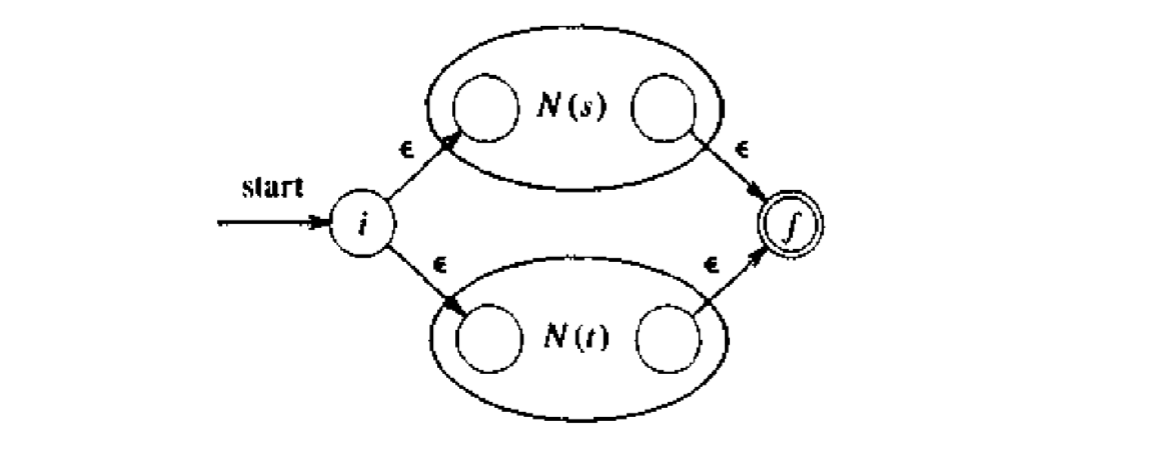
\includegraphics[width=\textwidth]{t_union}}
	\subfigure[]{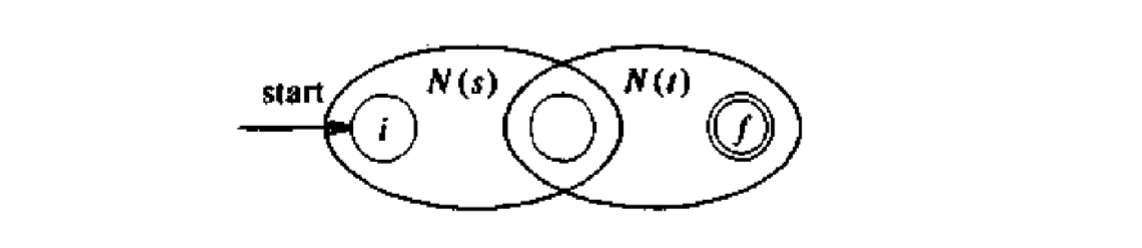
\includegraphics[width=\textwidth]{t_concatenacion}}
	\subfigure[]{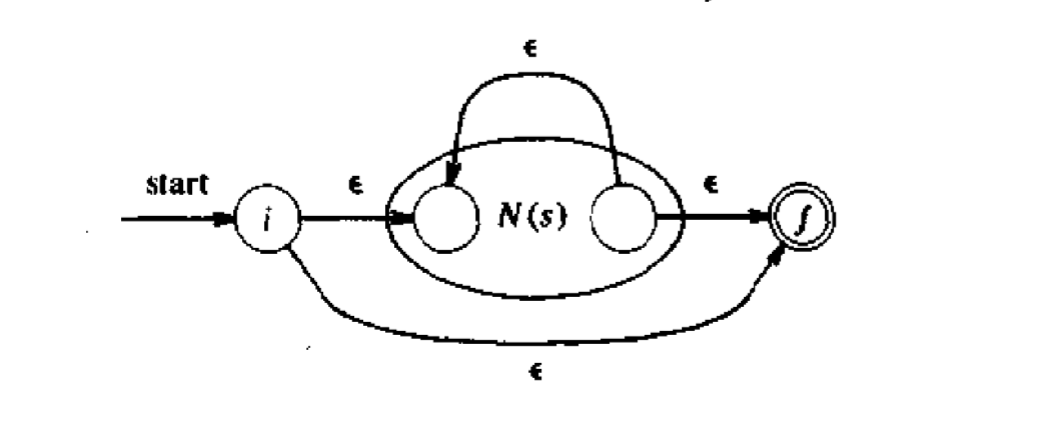
\includegraphics[width=\textwidth]{t_cerradura}}
	\caption{Conversiones de una ER a su respectivo AFN según el algoritmo de Thompson.}
	\label{fig:thompson}
\end{figure}








